\documentclass{article}
\usepackage[utf8]{inputenc}
\usepackage{graphicx}
\usepackage[T1]{fontenc}
\usepackage{circuitikz}
\usepackage[a4paper, margin=2.5cm]{geometry}
\usepackage{tikz}
\usepackage{array}
\definecolor{lightgray}{cmyk}{0,0,0,0.19}
\usetikzlibrary{positioning}
\begin{document}
	
\begin{titlepage}
	\centering
	\begin{figure}[h]
		\centering
		
\includegraphics[width=0.5\textwidth]{logo_polimi.png} 
	\end{figure}
	\vspace{1cm}
		\fbox{
			\begin{minipage}{\linewidth}
				\centering
				\vspace{1cm}
				{\LARGE\bfseries \textsc{Prova Finale}\par}
				{\LARGE\bfseries \textsc{Progetto di Reti Logiche}\par}
				\vspace{0.1cm}
				{\Large\itshape Prof. William Fornaciari \par}
				\vspace{0.5cm}
				{\Large\bfseries \textsc{Corso di laurea in Ingegneria Informatica}\par}
				{\large Anno accademico: 2023/2024 \par}
				\vspace{0.5cm}
				{\large\bfseries Alessandro Del Fatti\par}
				{\large Codice persona: 10790553 \par}
				\vspace{1cm}
			\end{minipage}
		}
	\vfill
	{\large Consegna del 01/04/2024\par}
	
\end{titlepage}

\section{Introduzione}
Il sistema progettato ha come scopo quello di ricevere in ingresso dei valori interi positivi, valutare la loro attendibilità e generare, in modo coerente con il valore letto, un ulteriore valore numerico che possa descriverne la credibilità. Si pensi, ad esempio, ad un sistema che opera in questo modo:
\begin{enumerate}
	\item Un sensore effettua una serie di misurazioni: sia $K$ il numero di misurazioni effettuate.
	\item Le $K$ misurazioni vengono mantenute in delle celle di memoria. Sia W il contenuto di ciascuna cella di memoria rappresentante una misurazione.
	\item Per ciascuna delle $K$ misurazioni si vuole dire se il valore memorizzato è attendibile oppure no. Si considerano attendibili valori di $W>0$ e non attendibili valori di $W=0$.
	\item Quindi, per ciascuna misurazione, si assegna un valore di credibilità $C$ secondo queste regole:
	\begin{enumerate}
		\item Se $W_i \neq 0$, il corrispondente valore di credibilità $C_i$ sarà massimo, cioè $C_i = 31$
		\item Se $W_i = 0$, la misurazione è da considerarsi non valida. Si sostituisce quindi il valore di $W_i$ con quello di $W_{i-1}$ e si pone $C_i$ a $C_{i-1} - 1$, se $C_{i-1} \geq 1$ altrimenti si pone $C_i = 0$. Se già il primo valore letto è nullo, cioè $W_0 = 0$, non si può «\textit{correggere}» con la lettura precedente e si mantengono $W_0= 0$ e  $C_0 = 0$.
	\end{enumerate}
\end{enumerate}
Il seguente schema esplicita in modo generale il principio di funzionamento del sistema e dove si colloca il componente progettato.
\begin{center}
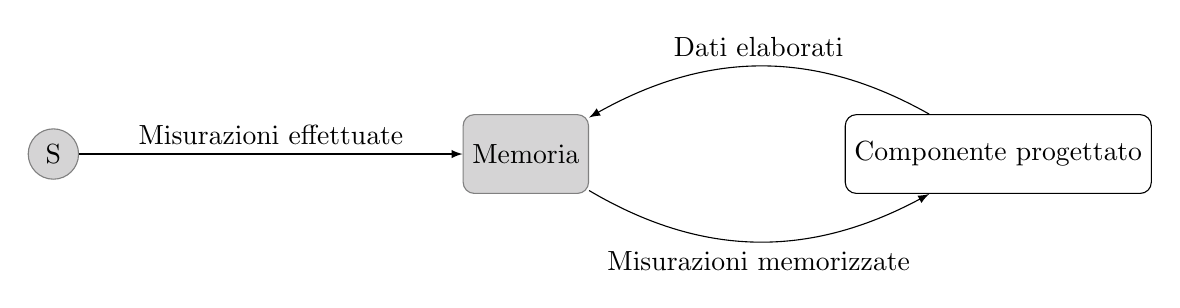
\begin{tikzpicture}[
	sensor/.style={circle, draw=gray, fill=lightgray, minimum width=0.5cm},
	component/.style={rectangle, draw, rounded corners, minimum width=1.5cm, minimum height=1cm},
	ram/.style={rectangle, draw=gray, fill=lightgray, rounded corners, minimum width=1.5cm, minimum height=1cm}, auto, node distance=6cm]
	\node[sensor] (S) at (0,0) {S};
	\node[ram, right of=S] (RAM) {Memoria};
	\node[component, right of=RAM](C) {Componente progettato};
	%\node[below =0.8cm of S] {\textsc{Sensore}};
	%\node[below =0.5cm of RAM] {\textsc{Memoria}};
	%\node[below =0.5cm of C] {\textsc{Componente Progettato}};
	\path[-latex, black] (S) edge[] node {Misurazioni effettuate} (RAM);
	\path[-latex, black] (RAM) edge[bend right] node[swap]{Misurazioni memorizzate} (C);
	\path[-latex, black] (C) edge[bend right] node[swap] {Dati elaborati} (RAM);
\end{tikzpicture}
\end{center}
Un esempio di elaborazione, con valori numerici, che racchiude le casistiche di input descritte è il seguente: 
\begin{table}[h]
	\centering
	\begin{tabular}{c|c||c}
		\textbf{Indirizzo}&\textbf{Valore pre-elaborazione}&\textbf{Valore post-elaborazione}\\
		\hline
		$ADD_1$&0&0\\
		$ADD_2$&0&0\\
		$ADD_3$&192&192\\
		$ADD_4$&0&31\\
		$ADD_5$&0&192\\
		$ADD_6$&0&30\\
	\end{tabular}
	\caption{Situazione della memoria pre e post-elaborazione}
\end{table}
\paragraph{Passo 1:} Elaborazione del primo valore
\begin{center}
\begin{tikzpicture}[
	component/.style={rectangle, draw, rounded corners, minimum width=1cm, minimum height=1cm},
	ram/.style={rectangle, draw=gray, fill=lightgray, rounded corners, minimum width=1cm, minimum height=1cm}, auto, node distance=6cm]
	\node[ram, right of=S] (RAM) {RAM - $ADD_1$};
	\node[component, right of=RAM](C) {Componente progettato};
	\path[-latex, black] (RAM) edge[bend right] node[swap]{$W_{ADD1}=0$} (C);
	\path[-latex, black] (C) edge[bend right] node[swap] {$W_{ADD1}=0,\quad C_{ADD2}=0$} (RAM);
\end{tikzpicture}
\end{center}
Leggo 0 dalla memoria. Si tratta del primo valore letto, quindi non posso «correggerlo» con quello letto al passo precedente.
\clearpage
\paragraph{Passo 2:} Elaborazione del secondo valore
\begin{center}
\begin{tikzpicture}[
	component/.style={rectangle, draw, rounded corners, minimum width=1.5cm, minimum height=1cm},
	ram/.style={rectangle, draw=gray, fill=lightgray, rounded corners, minimum width=1.5cm, minimum height=1cm}, auto, node distance=6cm]
	\node[ram, right of=S] (RAM) {RAM - $ADD_3$};
	\node[component, right of=RAM](C) {Componente progettato};
	\path[-latex, black] (RAM) edge[bend right] node[swap]{$W_{ADD3}=192$} (C);
	\path[-latex, black] (C) edge[bend right] node[swap] {$W_{ADD3}=192,\quad C_{ADD4}=31$} (RAM);
\end{tikzpicture}
\end{center}
Leggo 192 dalla memoria. Si tratta di un valore maggiore di 0, quindi lo considero attendibile e imposto al massimo il valore di credibilità $C=31$.
\paragraph{Passo 3:} Elaborazione del terzo valore
\begin{center}
\begin{tikzpicture}[
	component/.style={rectangle, draw, rounded corners, minimum width=1.5cm, minimum height=1cm},
	ram/.style={rectangle, draw=gray, fill=lightgray, rounded corners, minimum width=1.5cm, minimum height=1cm}, auto, node distance=6cm]
	\node[ram, right of=S] (RAM) {RAM - $ADD_5$};
	\node[component, right of=RAM](C) {Componente progettato};
	\path[-latex, black] (RAM) edge[bend right] node[swap]{$W_{ADD5}=0$} (C);
	\path[-latex, black] (C) edge[bend right] node[swap] {$W_{ADD5}=192,\quad C_{ADD6}=30$} (RAM);
\end{tikzpicture}
\end{center}
Leggo 0 dalla memoria. Non si tratta del primo valore letto, quindi non lo considero attendibile e riscrvo in memoria il valore di $W$ letto al punto precedente, ma abbasso il livello di credibilità: $C=30$.
\\
\\
I valori numerici di questo esempio sono coerenti con le specifiche: $K$, cioè il numero di letture che il componente deve effettuare, è esprimibile con 10 bit, $W$, il dato in memoria, è una parola da 8 bit e gli indirizzi di memoria sono da 16 bit.
\section{Architettura}
\begin{figure}[!ht]
	\centering
	\resizebox{1\textwidth}{!}{%
		\begin{circuitikz}
			\tikzstyle{every node}=[font=\large]
			\draw  (5,12.75) rectangle  node {\large K-REG} (8.75,10.25);
			\draw  (5,17.75) rectangle  node {\large ADDR-REG} (8.75,15.25);
			\draw  (5,7.75) rectangle  node {\large W-REG} (8.75,1.5);
			\draw  (12.5,6.5) rectangle  node {\large MUX} (15,2.75);
			\node [font=\large] at (13,6) {0};
			\node [font=\large] at (13,3.25) {1};
			\draw [->, >=Stealth] (1.25,16.5) -- (5,16.5)node[pos=0.5, fill=white]{16};
			\draw [->, >=Stealth] (1.25,11.5) -- (5,11.5)node[pos=0.5, fill=white]{10};
			\draw [->, >=Stealth] (1.25,4.75) -- (5,4.75)node[pos=0.5, fill=white]{8};
			\draw [->, >=Stealth] (8.75,5.75) -- (12.5,5.75)node[pos=0.5, fill=white]{8};
			\draw [->, >=Stealth] (8.75,3.25) -- (12.5,3.25)node[pos=0.5, fill=white]{5};
			\draw [->, >=Stealth] (15,4.75) -- (18.75,4.75)node[pos=0.5, fill=white]{8};
			\draw  (23.75,14) rectangle  node {\large FSM} (28.75,7.75);
			\draw [->, >=Stealth] (28.75,12.75) -- (32.5,12.75);
			\draw [->, >=Stealth] (28.75,9.25) -- (32.5,9.25);
			\draw [->, >=Stealth] (28,5.25) -- (28,7.75);
			\draw [->, >=Stealth] (26.75,5.25) -- (26.75,7.75);
			\node [font=\large] at (26.75,4.75) {CLK};
			\node [font=\large] at (28,4.75) {RST};
			\draw [->, >=Stealth] (28.75,11) -- (32.5,11);
			\draw [short] (27.5,14) -- (27.5,20.25);
			\draw [short] (27.5,20.25) -- (6.25,20.25);
			\draw [->, >=Stealth] (6.25,20.25) -- (6.25,17.75);
			\draw [short] (26.25,14) -- (26.25,19);
			\draw [short] (26.25,19) -- (7.5,19);
			\draw [->, >=Stealth] (7.5,19) -- (7.5,17.75);
			\draw [->, >=Stealth] (8.75,10.75) -- (23.75,10.75)node[pos=0.5, fill=white]{10};
			\draw [short] (25,14) -- (25,14.75);
			\draw [->, >=Stealth] (20,12) -- (23.75,12);
			\draw [short] (24.25,7.75) -- (24.25,1.5);
			\draw [short] (24.25,1.5) -- (14.5,1.5);
			\draw [->, >=Stealth] (14.5,1.5) -- (14.5,2.75);
			\draw [short] (25,7.75) -- (25,0.25);
			\draw [short] (25,0.25) -- (13,0.25);
			\draw [->, >=Stealth] (13,0.25) -- (13,2.75);
			\draw [->, >=Stealth] (5.25,9) -- (5.25,10.25);
			\draw [->, >=Stealth] (6.25,9) -- (6.25,10.25);
			\node [font=\large] at (5,8.75) {     CLK};
			\node [font=\large] at (6.5,8.75) {};
			\draw [->, >=Stealth] (5.25,14) -- (5.25,15.25);
			\draw [->, >=Stealth] (6.25,14) -- (6.25,15.25);
			\node [font=\large] at (5,13.75) {     CLK};
			\node [font=\large] at (6.25,13.75) { RST};
			\node [font=\large] at (6.25,8.75) { RST};
			\draw [->, >=Stealth] (6.25,0.25) -- (6.25,1.5);
			\draw [->, >=Stealth] (5.25,0.25) -- (5.25,1.5);
			\node [font=\large] at (5,0) {     CLK};
			\node [font=\large] at (6.25,0) {RST};
			\draw [short] (25,14.75) -- (7.5,14.75);
			\draw [->, >=Stealth] (7.5,14.75) -- (7.5,12.75);
			\draw [short] (23.75,13.75) -- (8.25,13.75);
			\draw [->, >=Stealth] (8.25,13.75) -- (8.25,12.75);
			\draw [short] (23.75,9.5) -- (7.5,9.5);
			\draw [->, >=Stealth] (7.5,9.5) -- (7.5,7.75);
			\draw [short] (23.75,8.75) -- (8.25,8.75);
			\draw [->, >=Stealth] (8.25,8.75) -- (8.25,7.75);
			\node [font=\large] at (20.75,12.25) {START};
			\node [font=\large] at (20.5,11) {K-IN};
			\node [font=\large] at (13.75,20.5) {EN-ADD-INC};
			\node [font=\large] at (14,19.25) {EN-ADD-READ};
			\node [font=\large] at (11.75,14) {EN-K-READ};
			\node [font=\large] at (11.75,15) {EN-K-DEC};
			\node [font=\large] at (18.25,1.75) {EN-MUX};
			\node [font=\large] at (18.25,0.5) {SEL-MUX};
			\node [font=\large] at (12,9.75) {EN-W-UPDATE};
			\node [font=\large] at (11.5,9) {FIRST-VAL};
			\node [font=\large] at (9.5,6) {OUT-W};
			\node [font=\large] at (9.5,3.5) {OUT-C};
			\node [font=\large] at (1.5,16.75) {ADDR};
			\node [font=\large] at (1.25,11.75) {K};
			\node [font=\large] at (1.25,5) {I-MEM-DATA};
			\node [font=\large] at (20.25,4.75) {O-MEM-DATA};
			\draw [->, >=Stealth] (8.75,16.5) -- (12,16.5)node[pos=0.5, fill=white]{16};
			\node [font=\large] at (13.75,16.5) {O-MEM-ADDR};
			\node [font=\large] at (29.7,13) {DONE};
			\node [font=\large] at (30,11.25) {MEM-EN};
			\node [font=\large] at (30,9.5) {MEM-WR};
		\end{circuitikz}
	}
	\caption{Schema a blocchi del componente progettato}
\end{figure}
Schema architetturale e degli stati della FSM. Per ogni componente breve descrizione e implementazione in VHDL.
\section{Risultati sperimentali}
Report timing e utilization di Vivado. Metodologia di testing ed elenco dei testbench.
\section{Conclusioni}
Cosa scrivo di bello qui????
\end{document}
